\documentclass[a4paper,12pt]{article}

\usepackage{graphicx}
\begin{document}
\pagenumbering{roman} 
\tableofcontents
 \newpage
 \pagenumbering{arabic}\newpage
\section{INTRODUCTION}
  \hspace{5mm}  
\subsection{ Project Profile}
\hspace{5mm}         
Photo sharing is an attractive feature which popularizes Online Social Networks (OSNs). Unfortunately, it may leak users.privacy if they are allowed to post, comment, and tag a photo freely. In this paper, we attempt to address this issue and study the scenario when a user shares a photo containing individuals other than himself/herself (termed co-photo for short). To prevent possible privacy leakage of a photo, we design a mechanism to enable each individual in a photo be aware of the posting activity and participate in the decision making on the photo posting. For this purpose, we need an efficient facial recognition (FR) system that can recognize.everyone in the photo. However, more demanding privacy setting may limit the number of the photos publicly available to train the
FR system. To deal with this dilemma, our mechanism attempts to utilize users’ private photos to design a personalized FR system specifically trained to differentiate possible photo co-owners without leaking their privacy. We also develop a distributed consensusbased
method to reduce the computational complexity and protect the private training set. We show that our system is superior to other possible approaches in terms of recognition ratio and efficiency. Our mechanism is implemented as a proof of concept Android
application on Facebook’s platform.
The main users in this system are:
\vspace{5mm}\newline
1.  ADMINISTATOR
\vspace{5mm}\newline
2.  USERS
\newpage
\section{ABOUT THE DEVELOPING TOOLS}  
\subsection{Introduction to JSP}
\hspace{5mm}       
 JSP technology is used to create dynamic web applications. JSP pages are easier to maintain then a Servlet. JSP pages are opposite of Servlets as a servlet adds HTML code inside Java code, while JSP adds Java code inside HTML using JSP tags. Everything a Servlet can do, a JSP page can also do it.
JSP enables us to write HTML pages containing tags, inside which we can include powerful Java programs. Using JSP, one can easily separate Presentation and Business logic as a web designer can design and update JSP pages creating the presentation layer and java developer can write server side complex computational code without concerning the web design. And both the layers can easily interact over HTTP requests. 
\newpage
\subsection{HeidiSQL}
HeidiSQL is a useful and reliable tool designed for web developers using the popular MySQL server, Microsoft SQL databases and PostgreSQL. It enables you to browse and edit data, create and edit tables, views, procedures, triggers and scheduled events. Also, you can export structure and data either to SQL file, clipboard or to other servers. Its codebase was originally taken from Ansgar Becker's own MySQL-Front 2.5 software. Due to having sold the MySQL-Front branding to an unrelated party, Becker chose "HeidiSQL" as a replacement. The name was suggested by a friend as a tribute to Heidi Klum, and was further reinforced by Becker's own nostalgia for Heidi, Girl of the Alps. HeidiSQL is a useful and reliable tool designed for web developers using the popular MySQL server, Microsoft SQL databases and PostgreSQL. It enables you to browse and edit data, create and edit tables, views, procedures, triggers and scheduled events. Also, you can export structure and data either to SQL file, clipboard or to other servers.

HeidiSQL is a free and open-source administration tool for MySQL and its forks, as well as Microsoft SQL Server and PostgreSQL. Its codebase was originally taken from Ansgar Becker's own MySQL-Front 2.5 software. Due to having sold the MySQL-Front branding to an unrelated party, Becker chose "HeidiSQL" as a replacement. The name was suggested by a friend as a tribute to Heidi Klum, and was further reinforced by Becker's own nostalgia for Heidi, Girl of the Alps.A version written in Java, jHeidi, was designed to work on Mac and Linux computers. It was discontinued in March 2010 in favor of Wine support.
\newpage
\section{SYSTEM ANALYSIS}
\hspace{5mm}
\subsection{Introduction }
\hspace{5mm}
System Analysis works with users to identify goals and build system to achieve them. System Analysis is an important phase of any system development process.  System analysis is a step-by-step process used to identify and develop or acquire the software need to control the processing of specific application. System analysis is a continuing activity the stages of the systems development. The system is studied to the minute’s details and analyzed. In analysis, a detailed study of these operation performed by a system and their relationships within and outside of the system is done
\vspace{5mm}\newline\par
The aim of the proposed system is to develop a system with improved facilities. The proposed system can overcome all the limitation of the existing system, such as student’s information is maintained in the database, it gives more security to data, ensures data accuracy, reduces paper work and save time, only eligible students get chance, it makes information flow efficient and paves way for easy report generation, reduce the space. proposed system is cost effective.        

\newpage
\subsection{Existing System}
\hspace{5mm}
Existing system is the facebook application.In which we can create an account, add friends, post our text and photos etc. But problem with the existing system is anyone can post their photos including our photos without our concern.So the security is one of the major problem
\newpage
\subsection{Limitations Of Existing System}
\hspace{5mm}
• security in photo tagging
Photo sharing is an attractive feature which popularizes Online Social Networks (OSNs). Unfortunately, it may leak users’ privacy if they are allowed to post, comment, and tag a photo freely. In this paper, we attempt to address this issue and study the scenario when a user shares a photo containing individuals other than himself/herself (termed co-photo for short). To prevent possible privacy leakage of a photo, we design a mechanism to enable each individual in a photo be aware of the posting activity and participate in the decision making on the photo posting. For this purpose, we need an efficient facial recognition (FR) system that can recognize everyone in the photo. However, more demanding privacy setting may limit the number of the photos publicly available to train the FR system. To deal with this dilemma, our mechanism attempts to utilize users’ private photos to design a personalized FR system specifically trained to differentiate possible photo co-owners without leaking their privacy. We also develop a distributed consensusbase method to reduce the computational complexity and protect the private training set. We show that our system is superior to other possible approaches in terms of recognition ratio and efficiency. Our mechanism is implemented as a proof of concept Android application on Facebook’s platform.
\newpage
\subsection{Feasibility Study}
\hspace{5mm}
       A feasibility study is needed to determine if a project or end result of a project is feasible and beneficial. The main objective of feasibility study is to test the technical, social and economic feasibility of developing a new computer system. Investigating the existing system in the areas under investigation and generating ideas about a new system does this. 
      The key considerations involved in the feasibility analysis are the following:
1.	Economic feasibility
2.	Technical feasibility
3.	Operational feasibility.
\subsubsection{Economic Feasibility}
\hspace{5mm}
Economic feasibility is a method for evaluating the effectiveness of a candidate system. This study is mainly concerned with cost-benefit analysis that is how much money the user is investing in any system and how much he is getting as a benefit in output. Our project is Economical Feasible because anyone uses this software would need only to buy the machine. Our hardware requirement is not too expensive. The money and human effort needed for the existing system is high .In the new system benefits outweigh costs. So as compare to cost the project is economically feasible.
We conduct an economic feasibility study for this exam seat mapping system and it also uses minimum hardware requirements that are already used in the existing system .In existing system manual records are used for storing details. The system is cost effective because of its compatibility and effort saving nature. The cost benefit ratio is very small and hence the proposed system is feasible.

\newpage
\subsubsection{Technical Feasibility}
\hspace{5mm}
 Technical feasibility includes whether the technology is available in the market for the development and its availability.  The assessment of technical feasibility must be based on an outline design of the system requirements in terms of input, output, files, programs and procedures. This study checks the technical aspects of system. Minimum requirements of the proposed system are a computer and internet connectivity, which will not add any additional expense in implementing the system. This software is simple to use and manage.Online Freelancer system also uses the minimum technologies for the creation of the web based application. The existing system has also required minimum technical requirements. So the proposed system is said to be technically feasible
\subsubsection{Operational Feasibility}
\hspace{5mm}
The new system is very much easier and user friendly than the existing system. It satisfies the requirements identified in the requirements analysis phase of system development. It reduces the operational time considerably. Operational cost is very less. The maintenance and modification of the new system needs very less human effort. Using command buttons throughout the application programs enhances the operational feasibility. The new system is operationally feasible and makes the operations simpler and quite easier.
The proposed system exam seat mapping system does not produce any problem to existing customers, organization etc. It reduces the drawback of existing system. All these reasons make the new system operationally feasible.
\newpage
\subsection{Proposed system}
\hspace{5mm}
The aim of the proposed system is to develop a system with improved facilities. The proposed system can overcome all the limitation of the existing system, such as student’s information is maintained in the database, it gives more security to data, ensures data accuracy, reduces paper work and save time, only eligible students get chance, it makes information flow efficient and paves way for easy report generation, reduce the space. proposed system is cost effective.
To debug the existing system, remove procedures those cause data redundancy, make navigational sequence proper. To provide information about audits on different level and also to reflect the current work status depending on organization/auditor or date. Password mechanism is used.In this paper, private information of a user is consideredas his/hers privacy and exposure policies; friend list and the private training data set Xa. In the rest of this subsection, we show how these private information are protected from a semi-honest adversary.
\vspace{5mm}\newline\par
We all know the importance of computerization. The world is moving ahead at lightning speed and everyone is running short of time. One always wants to get the information and perform a task he/she/they desire(s) within a short period of time and too with amount of efficiency and accuracy. The application areas for the computerization have been selected on the basis of following factors:

\newpage
 FEATURES 
\hspace{5mm}
           The proposed system is designed to eliminate all the drawbacks of the existing system. The system has been responsible for maintaining information about users, 
•	user registration, 
•	find friends 
•	add post
•	view friend request 
•	accept or reject friend request
•	messaging 
•	stress detection
•         view stressesd uers
Work changes and several ad hoc reports.
The major advantage of the proposed system is,
•	Centralized approach has a centralized FR engine in charge of recognizing all users over a large OSN..
•	One-against-all approach decompose the friendship graph and use our proposed consensus-based training method to perform collaborative training.
• One-against-one: The analysis of this approach is similar to the one-against-all approach, except that the average rounds in one training process should be much less, due to the fact that there are only two participants instead of D+ 1 ones.
\subsubsection{ Advantages of Proposed System }
\hspace{5mm}
•	There will be more data integrity.
•	photo tagging security
•	stress management
\newpage
\section{FACT FINDING TECHNIQUES}
\hspace{5mm}
The success of any project depends upon the accuracy of available data. Accurate information can be collected with the help of certain methods / techniques. These specific methods for finding information of the system are termed as fact finding techniques. Interview, Questionnaire, Record View and Observations are the different fact finding techniques used in this project. 
\subsection{Interview:}
\hspace{5mm}
This method is used to collect the information from groups or individuals. We select the people who are related with the system for the interview. In this method, we sit face to face with people and record their responses.
\subsection{Record View:}
\hspace{5mm}
The information related to the system is available in the source like company’s documents, websites and other records. This record review helped me to get valuable information about the system.
\subsection{Onsite observation: }
\hspace{5mm}
 Unlike the other fact finding techniques, in this method we visit the organization and observe and understand the working of the existing system, flow of the system, the users of the system etc.

\newpage
\section{ SYSTEM SPECIFICATION }
\hspace{5mm}
\subsection{Hardware Specification:- }
\hspace{5mm}
 The selection of hardware configuration is very important task related to software development. The processor should be powerful to handle all the operations. The hard disk should have the sufficient capacity to solve the database and the application.
 The hardware requirements for developing and implementing the proposed system are given below:
 Processor               -    Pentium –III
Speed                                -    1.1 Ghz
RAM                                 -    256  MB(min)
Hard Disk                          -   20 GB
Floppy Drive                     -    1.44 MB
Key Board                         -    Standard Windows Keyboard
Mouse                                -    Two or Three Button Mouse
\newpage
\subsection{Software Specification:-}
\hspace{5mm}
Windows XP server includes improved network, application, and Web services. It provides improved reliability and scalability, lowers yours cost of computing with powerful, flexible management services, and provides the best foundation for running business applications. It provides network data security by protecting data on the wire or at the network interface. It also provides stored data on the security by using data encryption. Data encryption is provided transparently within windows XP by feature known as Encrypting File System (EFS). It has the ability to run on a single PC chip with a user up to a multi-user, multi-processor network installation. The software requirements for developing and implementing the proposed system are given below:
               
	Operating System        	:   Windows 95/98/2000/NT4.0.

	Application  Server	           : Apache Tomcat 7.0.34.0
	Front End                     	:   HTML, Java.
	Scripts                           	:   JavaScript.
	Server side Script         	:   Java Server Pages.
	Database                        	:  HeidiSQL
	Database Connectivity 	:   JDBC.
\newpage
\subsubsection{HTML}
Hypertext Markup Language (HTML) is the standard markup language for creating web pages and web applications. With Cascading Style Sheets (CSS) and JavaScript it forms a triad of cornerstone technologies for the World Wide Web.[3] Web browsers receive HTML documents from a web server or from local storage and render them into multimedia web pages. HTML describes the structure of a web page semantically and originally included cues for the appearance of the document.

HTML elements are the building blocks of HTML pages. With HTML constructs, images and other objects, such as interactive forms, may be embedded into the rendered page. It provides a means to create structured documents by denoting structural semantics for text such as headings, paragraphs, lists, links, quotes and other items. HTML elements are delineated by tags, written using angle brackets. Tags such as <img /> and <input /> introduce content into the page directly. Others such as <p>...</p> surround and provide information about document text and may include other tags as sub-elements. Browsers do not display the HTML tags, but use them to interpret the content of the page.

HTML can embed programs written in a scripting language such as JavaScript which affect the behavior and content of web pages. Inclusion of CSS defines the look and layout of content. The World Wide Web Consortium (W3C), maintainer of both the HTML and the CSS standards, has encouraged the use of CSS over explicit presentational HTML since 1997.[4]
In 1980, physicist Tim Berners-Lee, a contractor at CERN, proposed and prototyped ENQUIRE, a system for CERN researchers to use and share documents. In 1989, Berners-Lee wrote a memo proposing an Internet-based hypertext system.[5] Berners-Lee specified HTML and wrote the browser and server software in late 1990. That year, Berners-Lee and CERN data systems engineer Robert Cailliau collaborated on a joint request for funding, but the project was not formally adopted by CERN. In his personal notes[6] from 1990 he listed[7] "some of the many areas in which hypertext is used" and put an encyclopedia first.

The first publicly available description of HTML was a document called "HTML Tags", first mentioned on the Internet by Tim Berners-Lee in late 1991.[8][9] It describes 18 elements comprising the initial, relatively simple design of HTML. Except for the hyperlink tag, these were strongly influenced by SGMLguid, an in-house Standard Generalized Markup Language (SGML)-based documentation format at CERN. Eleven of these elements still exist in HTML 4.
\newpage
HTML is a markup language that web browsers use to interpret and compose text, images, and other material into visual or audible web pages. Default characteristics for every item of HTML markup are defined in the browser, and these characteristics can be altered or enhanced by the web page designer's additional use of CSS. Many of the text elements are found in the 1988 ISO technical report TR 9537 Techniques for using SGML, which in turn covers the features of early text formatting languages such as that used by the RUNOFF command developed in the early 1960s for the CTSS (Compatible Time-Sharing System) operating system: these formatting commands were derived from the commands used by typesetters to manually format documents. However, the SGML concept of generalized markup is based on elements (nested annotated ranges with attributes) rather than merely print effects, with also the separation of structure and markup; HTML has been progressively moved in this direction with CSS.

\newpage

\subsubsection{java}

Java is a set of computer software and specifications developed by Sun Microsystems, which was later acquired by the Oracle Corporation, that provides a system for developing application software and deploying it in a cross-platform computing environment. Java is used in a wide variety of computing platforms from embedded devices and mobile phones to enterprise servers and supercomputers. Java applets, which are less common than standalone Java applications, run in secure, sandboxed environments to provide many features of native applications and can be embedded in HTML pages.
\vspace{5mm}\newline\par
Writing in the Java programming language is the primary way to produce code that will be deployed as byte code in a Java virtual machine (JVM); byte code compilers are also available for other languages, including Ada, JavaScript, Python, and Ruby. In addition, several languages have been designed to run natively on the JVM, including Scala, Clojure and Apache Groovy. Java syntax borrows heavily from C and C++, but object-oriented features are modeled after Smalltalk and Objective-C.[10] Java eschews certain low-level constructs such as pointers and has a very simple memory model where every object is allocated on the heap and all variables of object types are references. Memory management is handled through integrated automatic garbage collection performed by the JVM.
\vspace{5mm}\newline\par
On November 13, 2006, Sun Microsystems made the bulk of its implementation of Java available under the GNU General Public License (GPL). The latest version is Java 9, the second of the two supported (with e.g. security updates) versions as of 2017. Oracle (and others) has announced that using older versions (other than Java 8) of their JVM implementation presents serious risks, due to unresolved security issues.
\newpage
The heart of the Java platform is the concept of a "virtual machine" that executes Java bytecode programs. This bytecode is the same no matter what hardware or operating system the program is running under. There is a JIT (Just In Time) compiler within the Java Virtual Machine, or JVM. The JIT compiler translates the Java bytecode into native processor instructions at run-time and caches the native code in memory during execution.

The use of bytecode as an intermediate language permits Java programs to run on any platform that has a virtual machine available. The use of a JIT compiler means that Java applications, after a short delay during loading and once they have "warmed up" by being all or mostly JIT-compiled, tend to run about as fast as native programs.[16][17][18] Since JRE version 1.2, Sun's JVM implementation has included a just-in-time compiler instead of an interpreter. Although Java programs are cross-platform or platform independent, the code of the Java Virtual Machines (JVM) that execute these programs is not. Every supported operating platform has its own JVM.
\newpage

\subsubsection{java script}
JavaScript (/ˈdʒɑːvəˌskrɪpt/[6]), often abbreviated as JS, is a high-level, dynamic, weakly typed, prototype-based, multi-paradigm, and interpreted programming language. Alongside HTML and CSS, JavaScript is one of the three core technologies of World Wide Web content production. It is used to make webpages interactive and provide online programs, including video games. The majority of websites employ it, and all modern web browsers support it without the need for plug-ins by means of a built-in JavaScript engine. Each of the many JavaScript engines represent a different implementation of JavaScript, all based on the ECMAScript specification, with some engines not supporting the spec fully, and with many engines supporting additional features beyond ECMA.

As a multi-paradigm language, JavaScript supports event-driven, functional, and imperative (including object-oriented and prototype-based) programming styles. It has an API for working with text, arrays, dates, regular expressions, and basic manipulation of the DOM, but the language itself does not include any I/O, such as networking, storage, or graphics facilities, relying for these upon the host environment in which it is embedded.

Initially only implemented client-side in web browsers, JavaScript engines are now embedded in many other types of host software, including server-side in web servers and databases, and in non-web programs such as word processors and PDF software, and in runtime environments that make JavaScript available for writing mobile and desktop applications, including desktop widgets.

Although there are strong outward similarities between JavaScript and Java, including language name, syntax, and respective standard libraries, the two languages are distinct and differ greatly in design; JavaScript was influenced by programming languages such as Self and Scheme.
\newpage
\section{SYSTEM DESIGN }
\hspace{5mm}
\subsection{Introduction of System Design}     
\hspace{5mm}
In this project design technique used is top-down, object- oriented dynamic modeling technique. A top-down design approach starts by identifying the major components and iterating until the desired level of details is achieved. In object oriented design technique, the modules in the design represent data abstraction. A dynamic model aim to specify new the state of various objects changes as events occur
\subsection{Input Design }
\hspace{5mm}
 Input design is a part of overall system design, which requires very careful attention. Input design features can ensure the reliability of the system and produce result from accurate data, or they can result in the production or erroneous information. The input design also determines whether the user can interact efficiently with the system. 
Admin who was a person which they can add student to the system. placement Office who was manage the student details and can conduct the workshops for the students.
Company can register in this sytem and they can give their company details and company can conduct online exam,display the mark and select the students according to the mark...
also the students can register with their profile and they can attend online exams.view whether they are passed or not
\newpage
\subsection{Output Design}
\hspace{5mm}
One of the important features of an information system for users is the output produces. Output is the information delivered to users through the information system. Output design is very important phase because the output will be interactive manner. In order to create the most useful output possible. To make a user friendly output and for better communication the programmer can use the features of a window. 
admin can view the student details,comapny can view the student registerd for the vacancies and their informations.student can view the online exam results and vaccanices and related informations
\subsection{Database Design}
\hspace{5mm}
   Database design is the process of producing a detailed data model of database. This data model contains all the needed logical and physical design choices and physical storage The process of doing database design generally consists of a number of steps which will be carried out by the database designer. Usually, the designer must:
•	Determine the data to be stored in the database.
•	Determine the relationships between the different data elements.
•	Superimpose a logical structure upon the data on the basis of these relationships.
In this project database design generally the data is to be stored in the database whether it can more relation for each modules. And it provides the logical relation between them.
 \newpage
\subsection{Architectural Design}  
\hspace{5mm}
Architectural design is of crucial importance in software engineering during which the essential requirements like reliability, cost, and performance are dealt with. Architectural design is the responsibility of developers, some other people like user representatives, systems engineers, hardware engineers, and operations personnel are also involved. All these stakeholders must also be consulted while reviewing the architectural design in order to minimize the risks and errors.
\vspace{5mm}\newline\par
In Consumerfed is whole managed by the admin and regional office who was consulted the project on the requirements of the each user whether it will minimize the errors and risks.
\newpage
\subsection{System Modules}  
\hspace{5mm}
1. Admin module
The admin has the main role in the project. Admin manages the stresses user.and they can view all the users who share photos
\vspace{5mm}\newline
2.user module
in user module a user can create an account in the facebook,they can login to the facebook, edit their profile, view friends,add friends,add post,mesaggesing to friends etc.
\newpage
\subsection{Form Design}
\hspace{5mm}
 A form designing means deciding the contents and layout of forms for the purpose of collecting and processing the required information economically and efficiently. The importance of forms designing can be understood because of the following points:
1. Forms are used to collect record and communicate the required information according to the expectations of the needy persons. Therefore, forms are treated as tools of office work. If the forms are badly designed, it reduces the speed of operation of office work.
2. The forms create psychological impact on the people who use it. The people may be frustrated and get tired if the forms are not designed properly.
3. The badly designed forms results in more number of mistakes in clerical work. Hence, there is a need of well-designed forms to avoid mistakes in clerical work.
4. Sometimes, the designed form may project a poor image in the minds of the customers. This may adversely affect the good will of the company.
5. System is the basis for form design. Hence, forms are designed according to the needs of the system. If forms are badly designed, they can ruin a whole system.
6. The well-designed forms contribute much to the efficiency of employees of an organization and efficiency of the system.
7. The cost of forms is less than the cost of completing office forms, transporting and filling of office forms. The ratio will be greater if the forms are badly designed.  
\newpage
\subsection{Table Structure}
\hspace{5mm}
\begin{figure}[h!]
\includegraphics[scale=0.80]{m1.png}
\end{figure}
\begin{figure}[h!]
\includegraphics[scale=0.80]{m2.png}

\end{figure}
\newpage
\begin{figure}[h!]
\includegraphics[scale=0.80]{m4.png}

\end{figure}
\begin{figure}[h!]
\centering
\includegraphics[scale=0.80]{m3.png}

\end{figure}
\newpage
\begin{figure}[h!]
\centering
\includegraphics[scale=0.80]{m5.png}
\end{figure}
\begin{figure}[h!]
\includegraphics[scale=0.80]{m6.png}
\end{figure}
\newpage
\begin{figure}[h!]
\includegraphics[scale=0.80]{m7.png}
\end{figure}

\newpage
\subsection{UML}
\hspace{5mm}
\begin{figure}[h!]
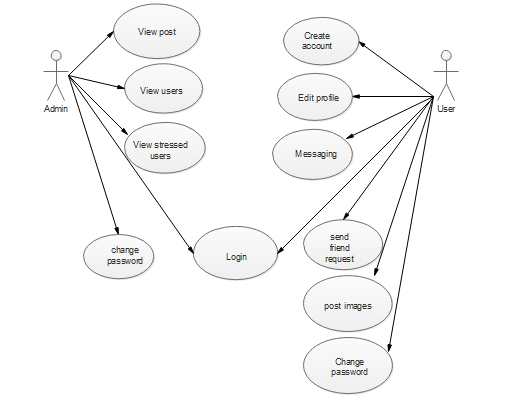
\includegraphics[scale=0.80]{uml1.png}
\end{figure}
\newpage
\hspace{5mm}
\begin{figure}[h!]
\includegraphics[scale=0.80]{activity.png}
\end{figure}
\newpage
\section{SYSTEM TESTING}
\hspace{5mm}
\subsection{Introduction to System Testing}
\hspace{5mm}
Testing is the process of examining the software to compare the actual behavior with that of the excepted behavior. The major goal of software testing is to demonstrate that faults are not present. In order to achieve this goal the tester executes the program with the intent of finding errors. Though testing cannot show absence of errors but by not showing their presence it is considered that these are   not present. 
\vspace{5mm}\newline\par
System testing is defined as the process by which one detects the defects in the software. Any software development organization or team has to perform several processes. Software testing is one among them. It is the final opportunity of any programmer to detect and rectify any defects that may have appeared during the software development stage. Testing is a process of testing a program with the explicit intention of finding errors that makes the program fail. In short system testing  and quality assurance is a review  in software products and related documentation for completion, correctness, reliability  and maintainability.
\vspace{5mm}\newline\par
System testing is the first stage of implementation, which is aimed at ensuring that the system works accurately and efficiently before live operation commences. Testing is vital to the success of the system. System testing makes a logical assumption that if all the parts of the system are correct and the goal will be successfully achieved. A series of testing are performed for the proposed system before the proposed system is ready for user acceptance testing.
\newpage
\subsection{Unit Testing}  
\hspace{5mm} 
This method of testing test the smallest unit of software called modules. It will test all the important path to find errors within the boundary of module. This has enabled the detection of errors in coding and logic.
 Various test cases are prepared. For each module these test cases are implemented and it is checked whether the module is executed as per the requirements and outputs the desired result. In this test each service input and output parameters are checked. In unit testing, All independent paths through the control structures are executed to ensure that all statements in the modules have been executed at least once. Error handling paths are also tested.
\subsection{Integration Testing}  
\hspace{5mm}
 Integration testing is a systematic technique for constructing the program structure while at the same time conducting tests to uncover errors associated with interfacing. In this testing, all individual modules were combined and module wise shifting was verified to be alright
 The integration testing is performed in the “Consumerfed” by combining the four modules.ie, by combining the admin, regional office, ration shop, suuplyco and triveni, user modules and found all modules are running without any error.
\newpage
\subsection{Validation Testing}  
\hspace{5mm}  
 Validation testing can be defined in many ways, but a simple definition is that validation succeeds when the software functions in manner that is reasonably accepted by user. Software validation is achieved through a series of tests that demonstrate conformity with requirement. Deviation or error discovered at this step in this project is corrected prior to completion of the project with the help of the user. In “Consumerfed” verifications are done correctly. So there is no chance for users to enter incorrect values. It will give error messages by using different validations. The validation testing is done very clearly and found it is error free.
 \subsection{Alpha Testing}  
\hspace{5mm}  
    Alpha testing is one of the most common software testing strategies used in software development. It’s specially used by product development organizations.
1.	This test takes place at the developer’s site. Developers observe the users and note problems.
2.	Alpha testing is testing of an application when development is about to complete. Minor design changes can still be made as a result of alpha testing.
3.	Alpha testing is typically performed by a group that is independent of the design team, but still within the company, e.g. in-house software test engineers, or software QA engineers.
4.	Alpha testing is final testing before the software is released to the general public. It has two phases:
5.	In the first phase of alpha testing, the software is tested by in-house developers. They use either debugger software, or hardware-assisted debuggers. The goal is to catch bugs quickly.
6.	In the second phase of alpha testing, the software is handed over to the software QA staff, for additional testing in an environment that is similar to the intended use.
7.	Alpha testing is simulated or actual operational testing by potential users/customers or an independent test team at the developers’ site. Alpha testing is often employed for off-the-shelf software as a form of internal acceptance testing, before the software goes to beta testing. 
\newpage
\subsection{Beta Testing}  
\hspace{5mm}  
Beta Testing is also known as field testing. It takes place at customer’s site. It sends the system/software to users who install it and use it under real-world working conditions.
•	A beta test is the second phase of software testing in which a sampling of the intended audience tries the product out. (Beta is the second letter of the Greek alphabet.) Originally, the term alpha testing meant the first phase of testing in a software development process. The first phase includes unit testing, component testing, and system testing. Beta testing can be considered “pre-release testing.
•	The goal of beta testing is to place your application in the hands of real users outside of your own engineering team to discover any flaws or issues from the user’s perspective that you would not want to have in your final, released version of the application. Example: Microsoft and many other organizations release beta versions of their products to be tested by users.
\subsection{Test Cases}  
\hspace{5mm}  
A Test Case is a script, program, or other mechanism that exercises a software component to ascertain that a specific correctness assertion is true. In general, it creates a specified initial state, invokes the tested component in a specified way, observes its behavior, and checks to ensure that the behavior was correct.
\newpage
\section{SYSTEM IMPLEMENTATION}  
\hspace{5mm}  
\subsection{Introduction to System Implementation}
The implementation is the final state and it is an important phase. It involves the individual programming; system testing, user training and the operational running of developed proposed system that constitutes the application subsystems. A major task of preparing for implementation is education of users, which should really have been taken place much earlier in the project when they were being involved in the investigation and design work. During the implementation phase system actually takes physical shape. In order to develop a system implemented planning is very essential. 
A software implementation method is a systematically structured approach to effectively integrate software based service or component into the workflow of an organizational structure or an individual end-user. This entry focuses on the process modeling (Process Modeling), a process model is a description of a process at the type level, side of the implementation of large product software, using the implementation of Enterprise Resource Planning systems as the main example to elaborate on. A product software implementation method is a blueprint to get users and/or organizations running with a specific software product. The method is a set of rules and views to cope with the most common issues that occur when implementing a software product: business alignment from the organizational view and acceptance from the human view. The implementation of product software, as the final link in the deployment chain of software production, is in a financial perspective of a major issue.
The implementation phase of the software development is concerned with translating design specification into source code. The user tests the developed system and changes are made according to their needs. Our system has been successfully implemented. Before implementation several tests have been conducted to ensure that no errors are encountered during the operation. The implementation phase ends with an evaluation of the system after placing into the operation for a period of time. Implementation is the third phase of the system processe. 
\newpage
\subsection{Training}
An analysis of user training focuses on two factors:
1.	User capabilities
2.	 Nature of the system to be installed.
Users range from the native to the highly sophisticated. They approach it as concrete learners, learning how to use the system without trying to understand which abstract principles determine which function. The distinction between concrete and formal (student type) learning says about what one can expect from trainees in general.These project also sophisticated the user capabilities and the corresponding nature of the system to be installed.
\newpage  
\subsection{Conversion}  
\hspace{5mm}  
Conversion refers to changing from one design to another system. The main objective of conversion is to put tested system into operation while holding costs, risks, and personal irritation to minimum. The various tasks involved in conversion are:
1	Creating computer compatible files.
2	Training the operating staffs.
3	Installing terminals and hardware.
The project entitled “Consumerfed” agreed the conversion phases that begin with a review of the project plan, the system test documentation and the implementation plan. And also conversion portion of the implementation plan is finalized and approved.  Files are converted.
\newpage
\subsection{Post Implementation Review}  
\hspace{5mm}
 Every system requires periodic evaluation after implementation. A post implementation review measures the system’s performance against predefined requirements. Unlike system testing, which determines where the system fails so that the necessary adjustments can be made, a post-implementation review determines how well the system continues to meet performances specifications. It is done after design and conversion are complete. It also provides information to determine whether major redesign is necessary. 
\newpage
\subsection{System Maintenance}  
\hspace{5mm}  
  Software maintenance is the modification of a software product after delivery to correct faults, to improve performance or other attributes. This section describes the six software maintenance processes as:
1. The implementation processes contains software preparation and transition activities, such as the conception and creation of the maintenance plan, the preparation for handling problems identified during development, and the follow-up on product configuration management. 
2. The problem and modification analysis process, which is executed once the application has become the responsibility of the maintenance group. The maintenance programmer must analyze each request, confirm it (by reproducing the situation) and check its validity, investigate it and propose a solution, document the request and the solution proposal, and, finally, obtain all the required authorizations to apply the modifications. 
3. The process considering the implementation of the modification itself. 
4. The process acceptance of the modification, by confirming the modified work with the individual who submitted the request in order to make sure the modification provided a solution. 
5. The migration process is exceptional, and is not part of daily maintenance tasks. If the software must be ported to another platform without any change in functionality, this process will be used and a maintenance project team is likely to be assigned to this task. 
6. Finally, the last maintenance process, also an event which does not occur on a daily basis, is the retirement of a piece of software. 
\newpage
\section{SYSTEM EVALUATION}  
\hspace{5mm}  
Although system evaluation is an ongoing process throughout the performance testing effort, it offers greater value when conducted early in the test project. The intent of system evaluation is to collect information about the project as a whole, the functions of the system, the expected user activities, the system architecture, and any other details that are helpful in guiding performance testing to achieve the specific needs of the project. 
1.	Your need to evaluate and select software that meets your business requirements.
2.	Your need to evaluate and select a partner that is capable of delivering the most benefit to your business from your software investment, as well as managing the risks inherent in system implementation projects.
3.	Your time and ours is valuable; at each step along the way we will each decide whether or not it is beneficial to proceed.
To help you with your selection, this evaluation process is designed to give us both a clear understanding of the systems to be implemented and the corresponding benefits of the partnership.This information provides a foundation for collecting the performance goals and requirements, characterizing the workload, creating performance-testing strategies and plans, and assessing project and system risks. A thorough understanding of the system under test is critical to a successful performance-testing effort. The measurements gathered during later stages are only as accurate as the models that are developed and validated in this stage. The evaluation provides a foundation for determining acceptable performance; specifying performance requirements of the software, system, or component(s); and identifying any risks to the effort before testing even begins. System evaluation providing in these project is needed to evaluate and select the requirements and managing the risk in system implementation on project. Also it is valuable in time so that way it is beneficial in each step.
\newpage
\section{CONCLUSION}  
\hspace{5mm}  
 The project was successfully completed within the time span allotted .The drawbacks of the existing system as listed before are fully evacuated. All the existing inconsistencies are fully solved as this system is implemented. This reduced the burden of the administration of the system. All the modules are tested separately and put together to form the main system. Finally the system is tested with real data and it worked successfully. Thus the system has fulfilled the entire objective defined.
The system has been developed in an interactive manner; the reports generated by the system are clear. The system is flexible, user friendly and has its own full data security and all data recovery facility. The developed system has mainly four modules admin , HOD, teacher, student. 
\newpage
\subsection{SCOPE FOR FUTURE ENHANCEMENTS}  
\hspace{5mm} 
In future we can expect the modified version of ‘facebook’. The system is very flexible for further up gradation with additional requirement of the self working, the jsp  and hidisql server makes this modifications very easily It is also possible to involve more functions into the system. This flexibility makes this system widening its scope. All day to day work can be done with much more ease and efficiency.
The database and the information can be updated to the latest coming versions. There are also possibilities for enhancing and further developing the project with the latest information and needs of the portal.
\newpage
\section{APPENDIX}  
\hspace{5mm} 
\subsection{APPENDIX A} 
\subsubsection{Sample Source Code / Pseudo Code}  
\hspace{5mm} 
\begin{verbatim}
\begin{itemsize}
\item COMPANY
\end{iemsize}
accet request
<%@page import="java.text.SimpleDateFormat"%>
<%@page contentType="text/html" pageEncoding="UTF-8"%>
<jsp:useBean class="com.myspace.dataaccess.DataAccess" id="con"/> 
<%@page  import="java.sql.*" %>
<%
String friendlistid=request.getParameter("friendlistId");
SimpleDateFormat format=new SimpleDateFormat("yyyy-MM-dd");
java.util.Date d=new java.util.Date();
String acceptedDate=format.format(d);
String update="update friendlist set status=1,accepteddate='"+acceptedDate+"' where friendlistid='"+friendlistid+"' ";
if(con.executeCommand(update))
{
    response.sendRedirect("viewfriendrequests.jsp?err=Request accepted successfully");
}else
{
    response.sendRedirect("viewfriendrequests.jsp?err=Server error while processing the request, please try again after some time.");
}
%>
change password
    <%@page contentType="text/html" pageEncoding="UTF-8"%>
<%@include  file="header.jsp" %>
<script src="../scripts/changeScript.js" type="text/javascript"></script>
<div class="section">
    <!-- box begin -->
    <div class="box">
        <div class="left-top-corner png"><div class="right-top-corner png"><div class="border-top png"></div></div></div>
        <div class="border-left png">
            <div class="border-right png">
                <div class="inside png">
                    <h2>Sign Up</h2>
                    <form id="registerForm" name="registerForm"  action="change_action.jsp">
                        <fieldset style="width:100%">
                            <div class="field"><label style="width: 100%"><%
                                String err = request.getParameter("err");
                                    %><%=(err == null ? "" : err)%></label></div>
                                    <div class="field"><label style="width:150px">Current password</label>&nbsp;<input class="fieldInput" type="password" name="txtCurrentpassword" /></div><span id="errCurrent" style="color: red"></span>
                            <div class="field"><label style="width:150px">New password</label>&nbsp;<input class="fieldInput" type="password" name="txtNewpassword" /></div><span id="errNew" style="color: red"></span>
                            <div class="field"><label style="width:150px">Confirm password</label>&nbsp;<input class="fieldInput" type="password" name="txtConfirmpassword" /></div><span id="errConfirm" style="color: red"></span>
                            <div class="wrapper">
                                <div style="padding-right: 229px" class="button"><span><span><input type="submit" value="Change passsword" onclick="return valid();"/></span></span></div>
                            </div>
                        </fieldset>
                    </form>
                </div>
            </div>
        </div>
        <div class="left-bot-corner png"><div class="right-bot-corner png"><div class="border-bot png"></div></div></div>
    </div>
    <!-- box end -->
</div>
<%@include  file="footer.jsp" %>   
 edit
 <%@page contentType="text/html" pageEncoding="UTF-8"%>
<!DOCTYPE html>
<%@include  file="header.jsp" %>
<script src="../scripts/profileScript.js" type="text/javascript"></script>
<div class="section">
    <!-- box begin -->
    <div class="box">
        <div class="left-top-corner png"><div class="right-top-corner png"><div class="border-top png"></div></div></div>
        <div class="border-left png">
            <div class="border-right png">
                <div class="inside png">
                    <h2>Sign Up</h2>
                    <form id="registerForm" name="registerForm" enctype="multipart/form-data" method="POST"   action="editimage_action.jsp">
                        <fieldset style="width:100%">
                           
                            <div class="field"><label><%
                                String err = request.getParameter("err");
                                    %><%=(err == null ? "" : err)%></label></div>
                                    <div class="field"><label>Choose image</label>&nbsp;<input class="fieldInput" type="file" name="flnImage"/></div>
                            
                            <div class="wrapper">
                                <div style="padding-right: 229px" class="button"><span><span><input type="submit" value="Update image" /></span></span></div>
                            </div>
                        </fieldset>
                    </form>
                </div>
            </div>
        </div>
        <div class="left-bot-corner png"><div class="right-bot-corner png"><div class="border-bot png"></div></div></div>
    </div>
    <!-- box end -->
</div>
<%@include  file="footer.jsp" %>
message
<jsp:useBean class="com.myspace.dataaccess.DataAccess" id="con"/> 
<%@page  import="java.sql.*" %>
<%
    String sel=request.getParameter("friendid");
    String name="";
    String id=session.getAttribute("UserID").toString();
    String se="select firstname from user where userid='"+sel+"'";
    ResultSet w=con.getData(se);
    if(w.next())
    { 
        name=w.getString("firstname");
    }
    
    String sele="select * from message  where (messagetouserid='"+sel+"' and Userid='"+session.getAttribute("UserID")+"') or (messagetouserid='"+session.getAttribute("UserID")+"' and Userid='"+sel+"')";
    ResultSet re=con.getData(sele);
    %>
<%@include file="header.jsp" %>

<div class="section">
    <!-- box begin -->
    <div class="box">
        <div class="left-top-corner png"><div class="right-top-corner png"><div class="border-top png"></div></div></div>
        <div class="border-left png">
            <div class="border-right png">
                <div class="inside png">
                    
                    <h2><%=name%></h2>
                    <div><%
                    String err=request.getParameter("err");
                    %><%=(err!=null?err:"")%></div>
                    <ul class="items-list">
                        <%
                            
                        while(re.next()){
                           String uid=re.getString("Userid");
                        %>
                        <h4></h4>
                        <%if(uid.equalsIgnoreCase(id))
                        {
                            %>
                     &nbsp;&nbsp;&nbsp;&nbsp;&nbsp;&nbsp;&nbsp;&nbsp;&nbsp;&nbsp;&nbsp;&nbsp;&nbsp;&nbsp;  &nbsp;&nbsp;&nbsp;&nbsp;&nbsp;&nbsp;&nbsp;&nbsp;&nbsp;&nbsp;&nbsp;&nbsp;&nbsp;&nbsp;&nbsp;&nbsp;&nbsp;&nbsp;&nbsp;&nbsp;  <textarea rows="4" cols="50" id="messagebox"  readonly="1"><%=re.getString("messagecontent")%></textarea>   
                                               <%
                        }
                        else{
                       %>
                     
                         
                       <textarea rows="4" cols="50" id="messagebox"  readonly="1"><%=re.getString("messagecontent")%></textarea>
                     <%
                        }
                        }
                       %> 
                       <form action="sendmessage.jsp">
                           
                        &nbsp;&nbsp;&nbsp;&nbsp;&nbsp;&nbsp;&nbsp;&nbsp;&nbsp;&nbsp;&nbsp;&nbsp;&nbsp;&nbsp;&nbsp;&nbsp;&nbsp;&nbsp;&nbsp;&nbsp; &nbsp; &nbsp; &nbsp; &nbsp; &nbsp; &nbsp; &nbsp;  <textarea rows="4" cols="50" id="messagebox" name="msg"></textarea>
                        <input type="hidden" name="id" value="<%=sel%>"/>
                        <br>
                        <input type="submit" value="Send" class="button"/>
                       </form>
                    </ul>
                      
                </div>
            </div>
             
        </div>
        <div class="left-bot-corner png"><div class="right-bot-corner png"><div class="border-bot png"></div></div></div>
    </div>
    <!-- box end -->
</div>
<%@include file="footer.jsp" %>

\end{verbatim}
\begin{verbatim}
\begin{itemsize}
\item course
\end{iemsize}

   
<%@page contentType="text/html" pageEncoding="UTF-8"%>
<jsp:useBean class="com.myspace.dataaccess.DataAccess" id="con"/> 
<%@page  import="java.sql.*" %>
<%
String selectUser="SELECT userid,firstname,lastname,emailID,contactnumber,gender from user where userid='"+session.getAttribute("UserID").toString()+"'";
ResultSet rsData=con.getData(selectUser);
rsData.next();
%>

<%@include  file="header.jsp" %>
<script src="../scripts/profileScript.js" type="text/javascript"></script>
<div class="section">
    <!-- box begin -->
    <div class="box">
        <div class="left-top-corner png"><div class="right-top-corner png"><div class="border-top png"></div></div></div>
        <div class="border-left png">
            <div class="border-right png">
                <div class="inside png">
                    <h2>Sign Up</h2>
                    <form id="registerForm" name="registerForm"  action="profile_action.jsp">
                        <fieldset style="width:100%">
                            <input type="hidden" value="register" name="hdnType"/>
                            <div class="field"><label><%
                                String err = request.getParameter("err");
                                    %><%=(err == null ? "" : err)%></label></div>
                            <div class="field"><label>First name</label>&nbsp;<input class="fieldInput" type="text" name="txtFirstName" value="<%=rsData.getString("firstname")%>"/></div><span id="errFirstName" style="color: red"></span>
                            <div class="field"><label>Last name</label>&nbsp;<input class="fieldInput" type="text" name="txtLastName" value="<%=rsData.getString("lastname")%>"/></div><span id="errLastName" style="color: red"></span>
                            <div class="field"><label>Contact number</label>&nbsp;<input class="fieldInput" type="text" name="txtContactNumber" value="<%=rsData.getString("contactnumber")%>"/></div><span id="errContactNumber" style="color: red"></span>
                            <div class="field"><label>Gender</label>&nbsp;
                            <%
                            if(rsData.getString("gender").equalsIgnoreCase("male")){
                            %>    
                                <input type="radio" name="rdbGender" value="Male" checked/>Male<input type="radio" name="rdbGender" value="Female"/>Female
                            <%
                            }else if(rsData.getString("gender").equalsIgnoreCase("femaile")){
                            %>
                            <input type="radio" name="rdbGender" value="Male" />Male<input type="radio" name="rdbGender" checked value="Female"/>Female
                            <%
                            }
                            %>
                            </div>
                            <div class="field"><label>EmailID</label>&nbsp;<input class="fieldInput" type="text" name="txtEmailID" value="<%=rsData.getString("emailid")%>"/></div><span id="errEmailID" style="color: red"></span>
                            <div class="wrapper">
                                <div style="padding-right: 229px" class="button"><span><span><input type="submit" value="Update profile" onclick="return valid();"/></span></span></div>
                            </div>
                        </fieldset>
                    </form>
                </div>
            </div>
        </div>
        <div class="left-bot-corner png"><div class="right-bot-corner png"><div class="border-bot png"></div></div></div>
    </div>
    <!-- box end -->
</div>
<%@include  file="footer.jsp" %> 
<%-- 
    Document   : viewposts
    Created on : Mar 22, 2015, 2:29:35 PM
    Author     : Dinesh
--%>

<%@page contentType="text/html" pageEncoding="UTF-8"%>
<jsp:useBean class="com.myspace.dataaccess.DataAccess" id="con"/> 
<%@page  import="java.sql.*" %>
<%

    String selectUser = "select p.title,p.postid,p.dateofupload,p.imageif,u.firstname,u.lastname,u.profImage "+
             " ,(select likestatus  from postlike where postid=p.postid and likeuserid='"+session.getAttribute("UserID").toString()+"') as likestatus "+
            " ,(select count(*) from postlike where postid=p.postid and likestatus=1) as likecount "+
            "  from post p inner join user u "+
            " on p.userid=u.userid where p.userid in(select fl.friendid from friendlist fl inner join user u on fl.friendid=u.userid where fl.userid='" + session.getAttribute("UserID").toString() + "' and status=1 "+
            " union "+
            " select fl.userid as friendid from friendlist fl inner join user u on fl.userid=u.userid where fl.friendid='" + session.getAttribute("UserID").toString() + "' and status=1) or p.userid='" + session.getAttribute("UserID").toString() + "' order by p.dateofupload desc";
    ResultSet rsUsers = con.getData(selectUser);
%>
<%@include  file="header.jsp" %>
<style>
    .visi{
        display:none;
    }
</style>
<script>
    $(document).ready(function(){
//        $('.commentDiv').css('display','none');
        $('.acomment').on('click',function(e){
            e.preventDefault();
            $.commentDiv=$(this).parents('table');
            $.commentDiv.find('.commentDiv').toggleClass('visi');
        });
        
        $('.SendComment').on('click',function(e){
            e.preventDefault();
            $.href=$(this).attr('href');
            $.comment=$(this).parents('table').find('.commentBox').val();
           window.location=$.href+'&&comment='+$.comment;
        });
        
        $('.showAll').on('click',function(e){
            e.preventDefault();
            $(this).parents('table').find('.subcomments').toggleClass('visi');
        });
        
        $('.like').on('click',function(e){
            e.preventDefault();
            $.href=$(this).attr('href');
            window.location=$.href;
        });
         $('.unlike').on('click',function(e){
            e.preventDefault();
            $.href=$(this).attr('href');
            window.location=$.href;
        });
    });
</script>
<!DOCTYPE html>
<div class="section">
    <!-- box begin -->
    <div class="box">
        <div class="left-top-corner png"><div class="right-top-corner png"><div class="border-top png"></div></div></div>
        <div class="border-left png">
            <div class="border-right png">
                <div class="inside png">
                    <div class="button"><span><span><a href="createpost.jsp" >Upload post</a></span></span></div>
                    <h2>Available posts</h2>
                    <div><%
                        String err = request.getParameter("err");
                        %><%=(err != null ? err : "")%></div>
                    <ul class="items-list">
                        <%
                            while (rsUsers.next()) {
                        %>
                        <li>
                            <table style="width:100%">
                                <tr>
                                    <td>
                                        <%
                                        if(!rsUsers.getString("imageif").equals("")){
                                        %>
                                        <img src="../posts/<%=rsUsers.getString("imageif")%>" alt="no post image" width="200px" height="200px"/>
                                        <%}%>
                                    </td>
                                </tr>
                                <tr>
                                    <td>
                                        <%=rsUsers.getString("title")%>
                                    </td>
                                </tr>
                                <tr>
                                    <td>
                                        <img alt="no image" src="../profImages/<%=rsUsers.getString("profImage")%>" width="50px" height="50px" />
                                        <h3><%=rsUsers.getString("firstname") + " " + rsUsers.getString("lastname")%></h3>
                                        <span>Uploaded on : <%=rsUsers.getString("dateofupload") %></span>
                                    </td>
                                </tr>
                                <tr>
                                    <td>
                                        <span class="likecount"><%=rsUsers.getString("likeCount")%></span>
                                        <%
                                        if(rsUsers.getString("likeStatus")==null || rsUsers.getString("likeStatus").equals("0")){
                                        %>
                                        <a href="like_action.jsp?postid=<%=rsUsers.getString("postid")%>&status=1" class="like">Like</a>
                                        <%
                                        }else{
                                        %>
                                        <a href="like_action.jsp?postid=<%=rsUsers.getString("postid")%>&status=0" class="unlike">Unlike</a>
                                        <%
                                        }
                                        %>
                                        <span style="float:right"><a href="#" class="acomment">Comment</a></span>
                                    </td>
                                </tr>
                                <tr>
                                    <td><a href="viewposts.jsp" >Hide comments</a></td>
                                </tr>
                                <%
                                String selectComment="select c.dateofcomment,c.comment,u.firstname,u.lastname,u.profimage from comment c inner join user u on c.commentuserid=u.userid where c.postid='"+request.getParameter("id")+"' order by c.dateofcomment desc";
                                ResultSet rsComments=con.getData(selectComment);
                                while(rsComments.next()){
                                %>
                                <tr>
                                    <td>
                                        <img alt="no image" src="../profImages/<%=rsComments.getString("profImage")%>" width="25px" height="25px" />
                                        <h3><%=rsUsers.getString("firstname") + " " + rsComments.getString("lastname")%></h3>
                                        <span><%=rsComments.getString("comment") %></span><br/>
                                        <span>Uploaded on : <%=rsComments.getString("dateofcomment") %></span>
                                    </td>
                                </tr>
                                <%
                                }
                                %>
                                
                                <tr class="visi commentDiv">
                                    <td>
                                        <textarea class="commentBox" rows="8" cols="80"></textarea><br/>
                                        <div class="button"><span><span><a href="sendcomment.jsp?postid=<%=rsUsers.getString("postid") %>" class="SendComment" >Post</a></span></span></div>
                                    </td>
                                    
                                </tr>
                            </table>
                            <div>
                            </div>
                        </li>
                        <%
                            }
                        %>
                    </ul>

                </div>
            </div>
        </div>
        <div class="left-bot-corner png"><div class="right-bot-corner png"><div class="border-bot png"></div></div></div>
    </div>
    <!-- box end -->
</div>

<%@page contentType="text/html" pageEncoding="UTF-8"%>
<jsp:useBean class="com.myspace.dataaccess.DataAccess" id="con"/> 
<%@page  import="java.sql.*" %>
<%

String selectUser="select fl.friendid,u.firstname,u.lastname,u.profImage from friendlist fl inner join user u on fl.friendid=u.userid where fl.userid='"+session.getAttribute("UserID").toString()+"' and status=1 "+
" union "+
" select fl.userid as friendid,u.firstname,u.lastname,u.profImage from friendlist fl inner join user u on fl.userid=u.userid where fl.friendid='"+session.getAttribute("UserID").toString()+"' and status=1";
ResultSet rsUsers=con.getData(selectUser);
%>
<%@include  file="header.jsp" %>
<script>
   
    $(document).ready(function(){
        $('#sendmessage').on('click',function(e){
            e.preventDefault();
            var message=$('#messagebox').val();
            if(message==''){
             alert('Please enter some message');
        }else
            {
                window.location=$(this).attr('href')+"&&message="+message+"&m=m";
            }
        });
    });
</script>
<!DOCTYPE html>
<div class="section">
    <!-- box begin -->
    <div class="box">
        <div class="left-top-corner png"><div class="right-top-corner png"><div class="border-top png"></div></div></div>
        <div class="border-left png">
            <div class="border-right png">
                <div class="inside png">
                    <%-- <textarea rows="8" cols="80" id="messagebox" name=></textarea>--%>
                    <h2>Users search result</h2>
                    <div><%
                    String err=request.getParameter("err");
                    %><%=(err!=null?err:"")%></div>
                    <ul class="items-list">
                        <%
                            if(rsUsers!=null){
                        while(rsUsers.next()){
                        %>
                        <li>
                            <img alt="no image" src="../profImages/<%=rsUsers.getString("profImage")%>" />
                            <h3><%=rsUsers.getString("firstname")+" "+rsUsers.getString("lastname")%></h3>
                            <%--  <div class="button"><span><span><a href="sendmessage.jsp?friendid=<%=rsUsers.getString("friendid")%>" id="sendmessage" >Send Your Message!</a></span></span></div>--%>
                        </li>
                       <%
                        }}else{
                       %>
                       <li>
                            <h3>No result</h3>
                        </li>
                       <%
                            }%>
                    </ul>

                </div>
            </div>
        </div>
        <div class="left-bot-corner png"><div class="right-bot-corner png"><div class="border-bot png"></div></div></div>
    </div>
    <!-- box end -->
</div>

<%@include  file="footer.jsp" %>
<%@include  file="footer.jsp" %>
<%@include file="AdminFooter.jsp" %>
package com.myspace.dataaccess;

import java.sql.Connection;
import java.sql.DriverManager;
import java.sql.ResultSet;
import java.sql.SQLException;
import java.sql.Statement;
import java.util.logging.Level;
import java.util.logging.Logger;

/**
 *
 * @author Dinesh
 */
public class DataAccess {

    Connection con = null;
    Statement st = null;
    ResultSet rs = null;

    public DataAccess() {
        try {
            Class.forName("com.mysql.jdbc.Driver");
            con = DriverManager.getConnection("jdbc:mysql://localhost/myspace", "root", "root");

        } catch (SQLException ex) {
            Logger.getLogger(DataAccess.class.getName()).log(Level.SEVERE, null, ex);
        } catch (ClassNotFoundException ex) {
            Logger.getLogger(DataAccess.class.getName()).log(Level.SEVERE, null, ex);
        }
    }

    public boolean executeCommand(String query) {
        boolean flag = false;
        try {
            st = con.createStatement();
            st.executeUpdate(query);
            flag = true;
        } catch (SQLException ex) {
            Logger.getLogger(DataAccess.class.getName()).log(Level.SEVERE, null, ex);
        } finally {
            return flag;
        }
    }

    public ResultSet getData(String query) {
        try {
            st = con.createStatement();
            rs = st.executeQuery(query);
        } catch (SQLException ex) {
            Logger.getLogger(DataAccess.class.getName()).log(Level.SEVERE, null, ex);
        } finally {
            return rs;
        }
    }

    public int getLength(ResultSet rs) {
        int count = 0;
        try {

            while (rs.next()) {
                count++;
            }
            rs.first();
        } catch (SQLException ex) {
            Logger.getLogger(DataAccess.class.getName()).log(Level.SEVERE, null, ex);
        } finally {
            return count;
        }
    }
}

<%@page contentType="text/html" pageEncoding="UTF-8"%>
<jsp:useBean class="com.myspace.dataaccess.DataAccess" id="con"/> 
<%@page  import="java.sql.*" %>
<%
String friendName=request.getParameter("q").replace("'", "''");
String selectUser="select *,(select count(*) from friendlist where friendid=u.userid AND userid='"+session.getAttribute("UserID")+"') as requested from user u where userid<>'"+session.getAttribute("UserID")+"' and ((firstname like '%"+friendName+"%' or lastname like '%"+friendName+"%'))";
ResultSet rsUsers=con.getData(selectUser);
%>
<%@include  file="header.jsp" %>
<!DOCTYPE html>
<div class="section">
    <!-- box begin -->
    <div class="box">
        <div class="left-top-corner png"><div class="right-top-corner png"><div class="border-top png"></div></div></div>
        <div class="border-left png">
            <div class="border-right png">
                <div class="inside png">

                    <h2>Users search result</h2>
                    <div><%
                    String err=request.getParameter("err");
                    %><%=(err!=null?err:"")%></div>
                    <ul class="items-list">
                        <%
                        while(rsUsers.next()){
                        %>
                        <li>
                            <img alt="no image" src="../profImages/<%=rsUsers.getString("profImage")%>" />
                            <h3><%=rsUsers.getString("firstname")+" "+rsUsers.getString("lastname")%></h3>
                            <%
                            if(rsUsers.getInt("requested")==0){
                            %>
                            <a href="incoming_request.jsp?friendId=<%=rsUsers.getString("userid")%>">Request as a friend</a>
                            <%}else%>
                        </li>
                       <%
                        }
                       %>
                    </ul>

                </div>
            </div>
        </div>
        <div class="left-bot-corner png"><div class="right-bot-corner png"><div class="border-bot png"></div></div></div>
    </div>
    <!-- box end -->
</div>

<%@page import="java.text.SimpleDateFormat"%>
<%@page contentType="text/html" pageEncoding="UTF-8"%>
<jsp:useBean class="com.myspace.dataaccess.DataAccess" id="con"/> 
<%@page  import="java.sql.*" %>
<%
    String m=request.getParameter("m");
String messagetouserid=request.getParameter("id");
String userid=session.getAttribute("UserID").toString();
String message=request.getParameter("msg");
SimpleDateFormat format=new SimpleDateFormat("yyyy-MM-dd");
java.util.Date d=new java.util.Date();
String dateofmessage=format.format(d);
String redirectPage=m==null?"viewfriends.jsp":"messages.jsp";
String insert="insert into message(userid,messagetouserid,messagecontent,dateofmessage)values('"+userid+"','"+messagetouserid+"','"+message.replace("'","''")+"','"+dateofmessage+"')";
if(con.executeCommand(insert))
{
    response.sendRedirect(redirectPage+"?err=Message sent");
}else
{
    response.sendRedirect(redirectPage+"?err=Server error while processing the request, please try again after some time.");
}

%>
<%@include  file="footer.jsp" %>
<%@page import="java.text.SimpleDateFormat"%>
<%@page contentType="text/html" pageEncoding="UTF-8"%>
<jsp:useBean class="com.myspace.dataaccess.DataAccess" id="con"/> 
<%@page  import="java.sql.*" %>
<%
String postid=request.getParameter("postid");
String status=request.getParameter("status");
String userid=session.getAttribute("UserID").toString();
SimpleDateFormat format=new SimpleDateFormat("yyyy-MM-dd");
java.util.Date d=new java.util.Date();
String dateoflike=format.format(d);

String selectCount="Select count(*) as c from postlike where postid='"+postid+"' and likeuserid='"+userid+"'";
ResultSet rsData=con.getData(selectCount);
if(rsData.next() && rsData.getInt("c")>0){
    String update="update postlike set likestatus='"+status+"' where  postid='"+postid+"' and likeuserid='"+userid+"'";
    if(con.executeCommand(update))
    {
        response.sendRedirect("viewposts.jsp");
    }else
    {
        response.sendRedirect("viewposts.jsp?err=Server error while processing the request, please try again after some time.");
    }
}else
{
    String insert="insert into postlike(postid,likeuserid,dateoflike)values('"+postid+"','"+userid+"','"+dateoflike+"')";
    if(con.executeCommand(insert))
    {
        response.sendRedirect("viewposts.jsp");
    }else
    {
        response.sendRedirect("viewposts.jsp?err=Server error while processing the request, please try again after some time.");
    }
}

%>

<%@page contentType="text/html" pageEncoding="UTF-8"%>
<jsp:useBean class="com.myspace.dataaccess.DataAccess" id="con"/> 
<%@page  import="java.sql.*" %>

<%@page import="java.text.SimpleDateFormat"%>
<%@page import="java.io.File"%>
<%@page import="java.sql.*" %>
<%@page import="java.util.*" %>
<%@page import="java.io.*" %>
<%@page import="org.apache.commons.fileupload.*" %>
<%@page import="org.apache.commons.fileupload.servlet.*" %>
<%@page import="org.apache.commons.fileupload.disk.*" %>

<%

    String title="";
    String filename="";
    String userid=session.getAttribute("UserID").toString();
   SimpleDateFormat format=new SimpleDateFormat("yyyy-MM-dd");
java.util.Date d=new java.util.Date();
String dateofupload=format.format(d);
    FileItem f_item = null;
    File proj_path = new File(config.getServletContext().getRealPath("/"));
    String file_path = proj_path.getParentFile().getParentFile().getPath() + "\\web\\posts\\";
//checking if request cotains multipart data
    boolean isMultipart = ServletFileUpload.isMultipartContent(request);

    if (isMultipart) {

        FileItemFactory factory = new DiskFileItemFactory();
        ServletFileUpload upload = new ServletFileUpload(factory);

        //declaring a list of form fields
        List items_list = null;

        //assigning fields to list 'items_list'
        try {
            items_list = upload.parseRequest(request);
        } catch (FileUploadException ex) {
            out.println(ex);
        }

        //declaring iterator
        Iterator itr = items_list.iterator();

        //iterating through the list 'items_list'
        while (itr.hasNext()) {
            //typecasting next element in items_list as fileitem
            f_item = (FileItem) itr.next();
            if (f_item.isFormField()) {
                if (f_item.getFieldName().equalsIgnoreCase("txtTitle")) {
                    title = f_item.getString();
                }
            } else {
                try {
                    if (f_item.getFieldName().equalsIgnoreCase("flnPost")) {
                        filename = f_item.getName();
                        File savedFile1 = new File(file_path + filename);
                        f_item.write(savedFile1);
                    }

                } catch (Exception e) {
                }
            }
        }

    }
   String insertPost="insert into post(userid,title,dateofupload,imageif)values('"+userid+"','"+title+"','"+dateofupload+"','"+filename+"')";
   if(con.executeCommand(insertPost)){
       response.sendRedirect("createpost.jsp?err=Post uploaded successfully");
   }else
   {
       response.sendRedirect("createpost.jsp?err=Server error while processing the request, please try again after some time");
   }

%>
\end{verbatim}
\newpage
\subsection{APPENDIX B} 
\subsubsection{SCREEN SHOTS}  
\hspace{5mm} 
\begin{enumerate}
\item create new account
\begin{figure}[h!]
\includegraphics[scale=0.60]{h1.png}
\end{figure}
\newpage
\item login
\begin{figure}[h!]
\includegraphics[scale=0.60]{h2.png}
\end{figure}
\newpage
\item edit profile
\begin{figure}[h!]
\includegraphics[scale=0.60]{profile.png}
\end{figure}
\newpage
\item  upload post
\begin{figure}[h!]
\includegraphics[scale=0.60]{post.png}
\end{figure}
\newpage
\item  admin login
\begin{figure}[h!]
\includegraphics[scale=0.60]{login.png}
\end{figure}
\newpage
\item  view users
\begin{figure}[h!]
\includegraphics[scale=0.60]{view.png}
\end{figure}
\newpage
\item  search results
\begin{figure}[h!]
\includegraphics[scale=0.60]{search.png}
\end{figure}
\end{enumerate}
\newpage
\subsection{APPENDIX C} 
\begin{thebibliography}{10}
\bibitem{latexGuide} Manjush Talmale, Abhishek Kinhekar, Akshay Saraf, Milind Bhajan “Mobile Phone Cloning: History, Present Scenario and Precautionary  Techniques”, Nagpur, 2013International Journal of Application  or  Innovation in Engineering and  Management (IJAIEM) 2013 
 \bibitem{latexGuide}\texttt{http://www.google.co.in}.
 \bibitem{latexMath}\texttt{http://www.wikipedia.org}.
 \bibitem{latexGuide}\texttt{http://www.seminarsonly.com}.
 \bibitem{latexGuide}\texttt{http://www.1000projects.org/}.
 \end{thebibliography}
\end{document}